\chapter{APT}
\label{cha:7}
%\documentclass[10pt]{article}\

%%%%%%%%%%%%%%%%%%%%%%%%%%%%%%%%%%%%%%%%%%%%%%%%%%%%%%%%%%
%%%%%			Introduction Chapter 7			%%%%%%
%%%%%												%%%%%%
%%%%%												%%%%%%
%%%%%%%%%%%%%%%%%%%%%%%%%%%%%%%%%%%%%%%%%%%%%%%%%%%%%%%%%%


\section{Advanced Persistent Threats}

A targeted attack follows most of the time a serie of stages to attack its victim. This pattern of stages is also know as the Kill Chain, first mentioned by .. []. An APT will not always follow exact each step of this chain but it will give a good guideline of how an APT works. 
\begin{enumerate}
\item \textbf{Reconnaissance}: During the first step of the Kill Chain an attacker will look for information to find an interesting victim. This information can be emailaddresses, IP addresses, conference information, anything that is available about the victim.
\item \textbf{Weaponization}: In the second stage the attacker will use an exploit and add a malicious playload to be send to the victim. 
\item \textbf{Delivery}: The attacker will deliver his malicious code to the victim through different kins of intrusion methods. This can include email, usb stick, cd's, web, applications or other means.
\item \textbf{Exploitation}:The attacker executes the exploit, which is only relevant if the attacker uses an exploit.
\item \textbf{Installation}: The malware will be installed on the asset. This is only relevant if the attacker uses malware as a part of the attack.
\item \textbf{Command and Control}: The attacker will set up a command and control channel for remote manipulation of the victim.
\item \textbf{Actions on Objectives}: With ''hands on keyboard'' access, intruders accomplish their original goal. 
\end{enumerate}
\todo{nog uitbreiden, toevoegen that attackers will stay unnoticed for as long as possible or leave unnoticed with sensitive information}

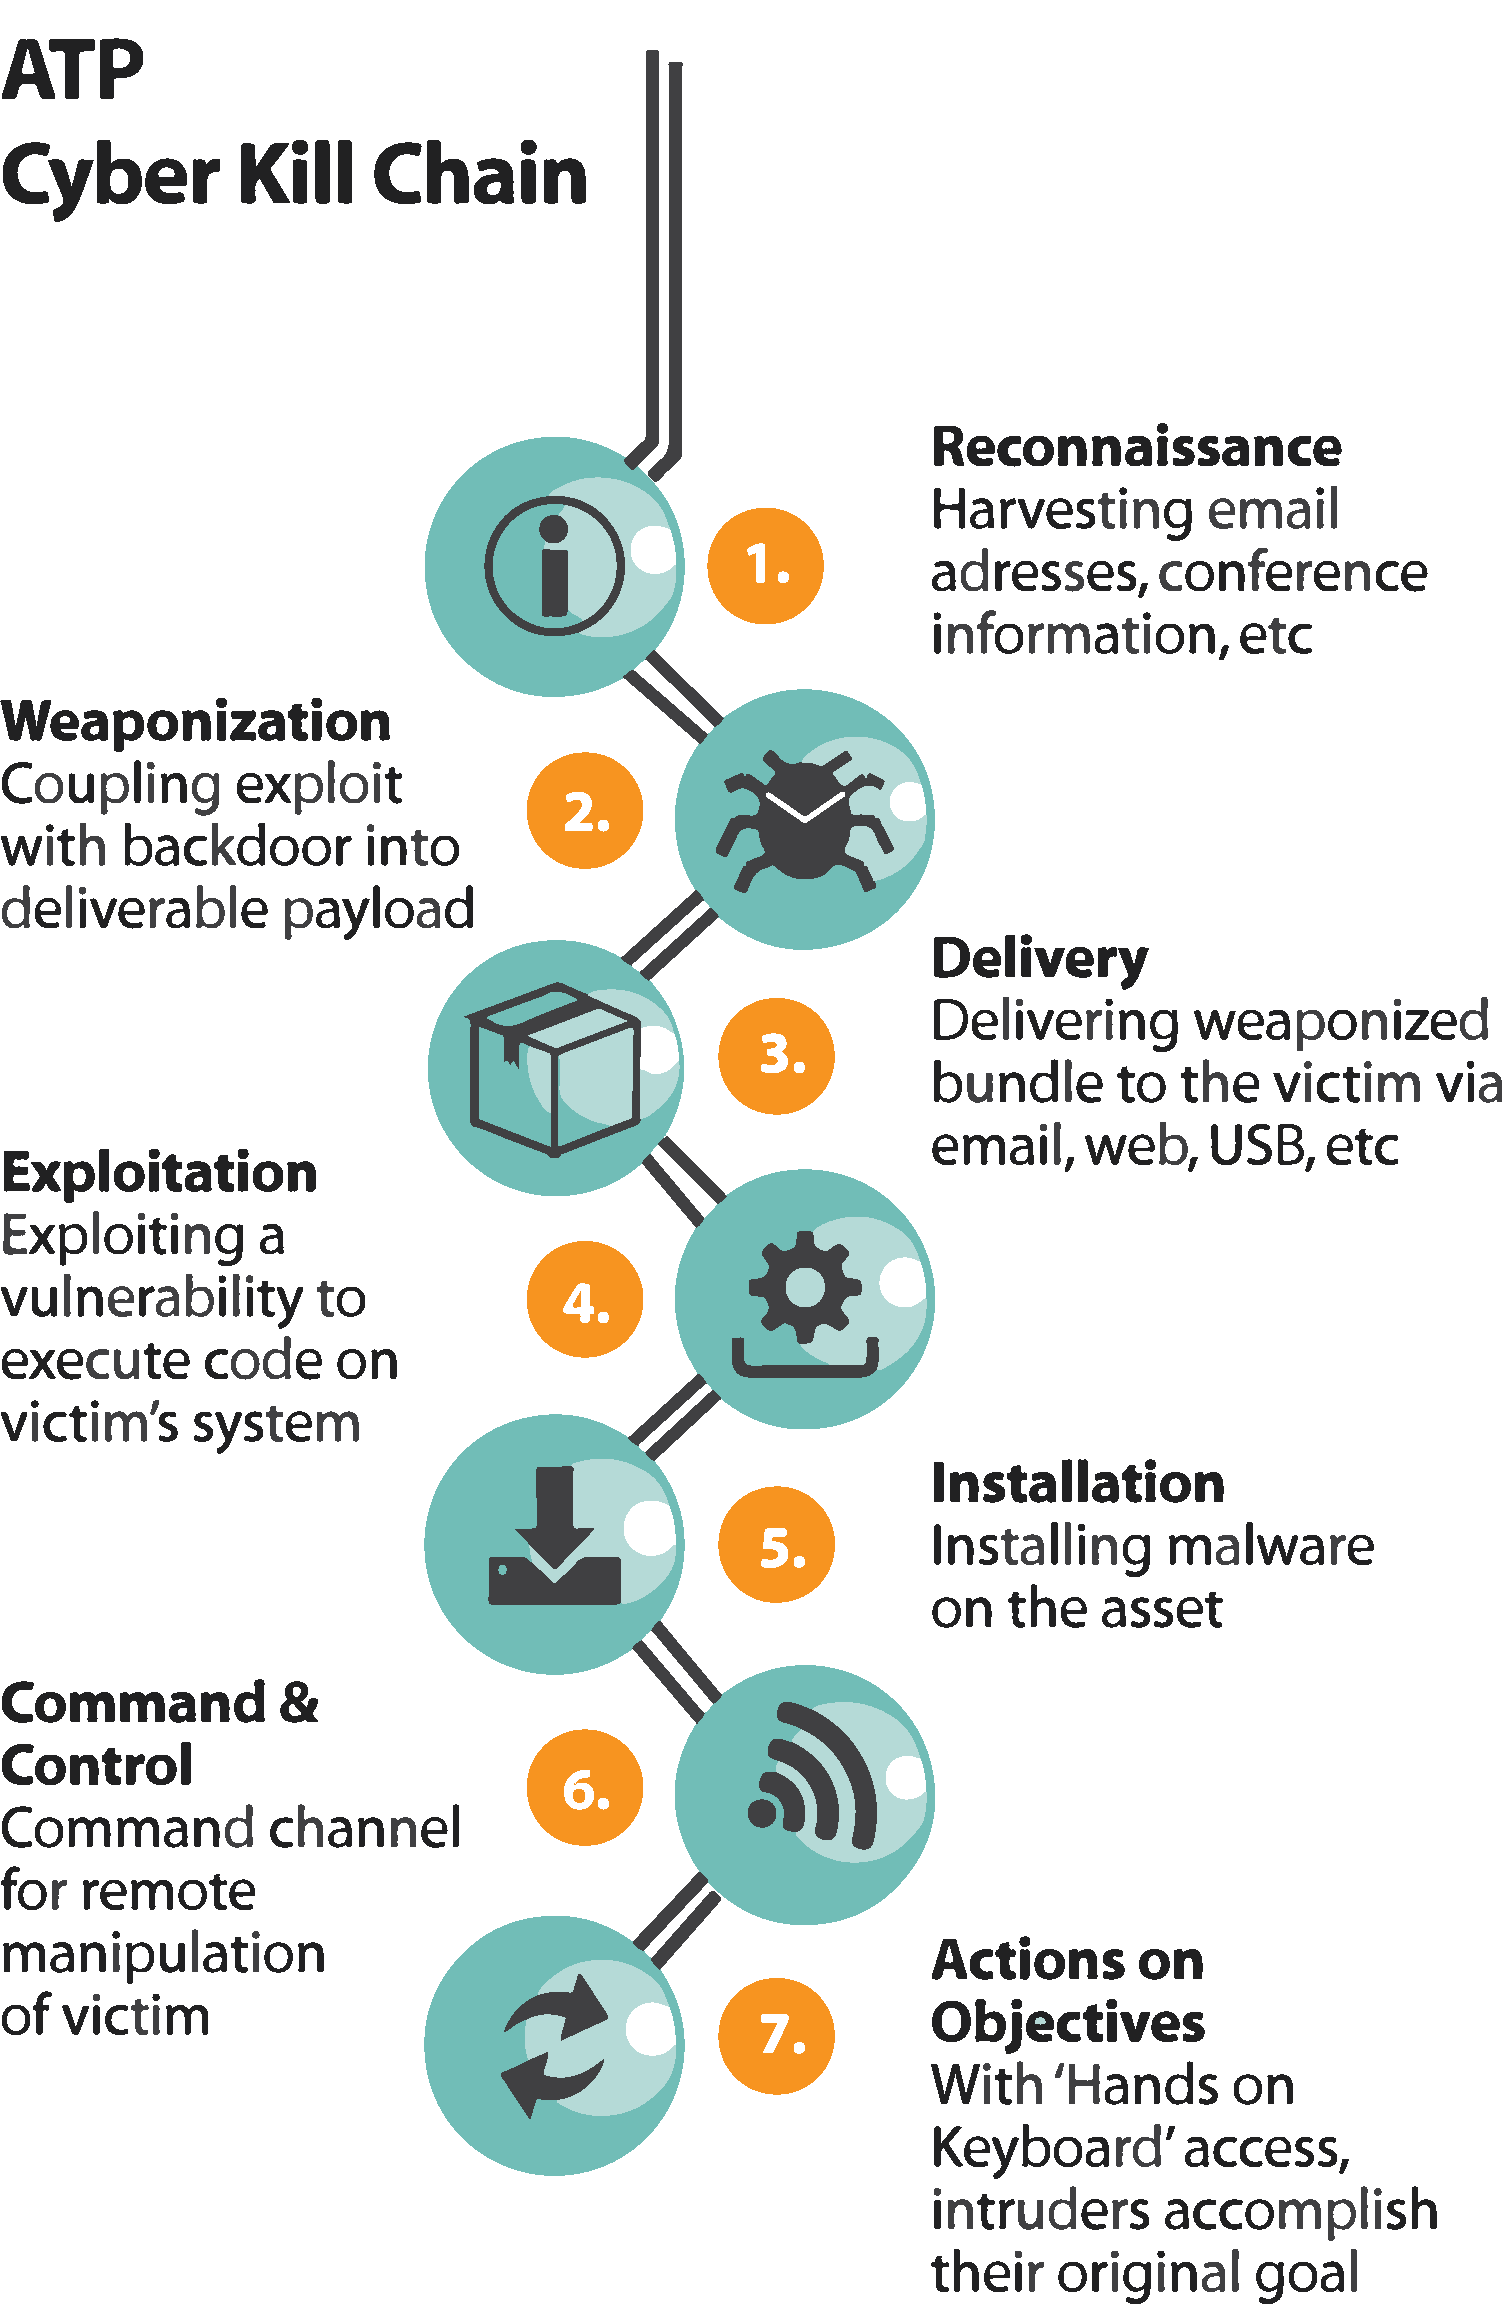
\includegraphics[scale=0.7]{Images/chainAPT} 